%
%	WISS 2015サンプルファイル (未来ビジョンテンプレート, 最後数行空き問題解決バージョン)
%
%	2010/07/12 Ver 1.0 秋田 純一
%	2010/08/04 Ver 1.1 後藤 真孝
% 	2011/09/27  Ver 1.4 渡邊 恵太 (協力:五十嵐悠紀)
% 	2015/02/08  Ver 1.5 大槻 麻衣
% 	2016/05/26  Ver 1.6 大槻 麻衣


\documentclass[twoside]{wiss}

\usepackage{ascmac}
\usepackage[dvips]{graphicx}
\usepackage{nidanfloat} %% appended in WISS2010 for Future Vision (2010/7/7:akita)
\usepackage{multicol}
%\usepackage{color,array}
%\usepackage{boxedminipage}

%% balance.styを追加 (2012/9/27:watanabe, Igarashi)
\usepackage{balance}    %% 最後のページの高さを揃えるために追加  (2012/9/27:watanabe, Igarashi)
%%% 最後のページの2段組の高さを揃える.\balanceを入れる.
%%% そろえたくないときは,\nobalance

%% urlのOverflow対策
\usepackage{url}

\journalhead{WISS論文タイトル} %%%%%% ←← 著者において必ず記入すること

\begin{document}

\title{WISS論文タイトル}
\etitle{}%2012年では英文タイトルは廃止されました.記入しないでください.
%
%注意
%
%
% WISS2016かラシングルブラインドとなりました.投稿時に氏名と所属を記入してください.
\author{鈴木 太郎\affil{○×大学} \affil{株式会社○○}  高橋 花子\affil{○△大学}
  佐藤 次郎\affil{○△大学}  田中 三郎\affil{株式会社○○}
  渡邊 四郎\affil{○△大学}  伊藤 五郎${}^* {}^\dag {}^\ddag {}^\mathsection
{}^\mathparagraph$}

\begin{abstract}
概要は和文400文字程度で書く.(WISS2014より600字程度から400字程度となった)
概要サンプル 概要サンプル 概要サンプル 概要サンプル 概要サンプル 概要サンプル
概要サンプル 概要サンプル 概要サンプル 概要サンプル 概要サンプル 概要サンプル
概要サンプル 概要サンプル 概要サンプル 概要サンプル 概要サンプル 概要サンプル
概要サンプル 概要サンプル 概要サンプル 概要サンプル 概要サンプル 概要サンプル
概要サンプル 概要サンプル 概要サンプル 概要サンプル 概要サンプル 概要サンプル
概要サンプル 概要サンプル 概要サンプル 概要サンプル 概要サンプル 概要サンプル
概要サンプル 概要サンプル 概要サンプル 概要サンプル 概要サンプル 概要サンプル
概要サンプル 概要サンプル 概要サンプル 概要サンプル 概要サンプル 概要サンプル
概要サンプル 概要サンプル 概要サンプル 概要サンプル
\end{abstract}

\maketitle

\section{はじめに}

このLatex2e用スタイルクラスは,WISS 2016 における
論文投稿用である.2014年からはWordテンプレートを用意した.
著者各位においては,WISS のホームページ\cite{wiss}
および以下の注意を熟読して効率的な論文執筆をされるよう望む.
やむをえず他の手段で原稿を書く場合は,
限りなく同じ形式に仕上げること.
著しく異なる形式の場合,不採録の理由となる場合がある.

\section{論文執筆について}

\subsection{全般的な注意事項}

このスタイルクラスを利用するには,\verb|wiss.cls|,
\verb|wissbase11.cls|,\verb|jwiss.bst|をコンパイラが参照できるパスに置
く.通常は\TeX 文書ファイルと同じディレクトリに置けば自動的に参照される.
また\TeX 文書の先頭にある\verb|\documentclass|で\verb|wiss|を指定する.
全体としては右の枠線内のようになる.

論文の文体は「だ」「である」調,句読点は「,」「.」を強く推奨する.図の
レイアウトなどの特別な場合を除いて本文は2段組とする.原稿は
\textgt{A4サイズpdf出力}し,上下左右のマージンは厳守しなければな
らない.また,ページ数は必ず規定のページ数でなければならない.
まれにレターサイズになってしまっている原稿があるため要注意.

Overfull (規定の枠内からはみ出して文字を書くこと)してはならない.本文中
や参考文献で長いURLなどを書き入れると,
\verb|http://www.sample.url.xx.yyy/| のようにOverfullが発生することがあ
る.必ず仕上がりを確認し,このようなことが起きないように文章を調整する.
URLの場合は\verb|\url{}|を使うことによって適切な個所で改行される.
はみ出した部分については編集者において削除することがある.

\begin{screen}
\begin{verbatim}
\documentclass[twoside]{wiss}
.....
\journalhead{...}
\begin{document}
\title{...}
\etitle{...}
\author{...
    \affil{...}}
\begin{abstract}
.....
\end{abstract}
\maketitle
\section{...}
本文...

\bibliographystyle{jwiss}
\bibliography{...}

\begin{figure*}[!b]
未来ビジョン関連のlatex記述
\end{figure*}
\end{verbatim}
\end{screen}



\subsection{表題,著者名,著者所属,概要}

和文タイトルを\verb|\title{}|と\verb|\journalhead{}|の\underline{\textbf{両方に}}書く.
\verb|\journalhead{}|に書かれたタイトルは3ページ目以降の奇数ページの
ヘッダ(ハシラ)として現れる.この際,必ず表題と同じになっているかを確認すること.
また,1ページ目のタイトルは右側の余白にはみ出さないように注意する.

\begin{figure}[htp]
\centering
\setlength{\unitlength}{1mm}
\begin{picture}(90,30)
\put(50,8){\line(0,1){16}}
\put(15,22){\vector(1,0){35}}
\put(15,23){\small \textbf{はみださないように}}

\put(0,15){\makebox(50,3){\small per Dooper Title Styling System}}
\put(0,0){\makebox(50,10)[tr]{る場合,著者は必ず仕上がりを}}
\put(0,0){\makebox(50,6)[tr]{奇数ページのヘッダ(ハシラ)が}}
\put(0,0){\makebox(50,2)[tr]{を同じ意味の短い表現に改める}}

\multiput(70,0)(0,2){15}{\line(0,1){1}}
\multiput(0,30)(2,0){35}{\line(1,0){1}}

\put(52,27){\tiny (奇数ページ右上)}
\put(55,15){\small ヘッダ(ハシラ)}
\put(55,0){\makebox(8,10)[l]{\small 本文}}
\end{picture}
\caption{ヘッダの例}
\label{figure:header}
\end{figure} 

原稿を作成する場合,著者は必ず仕上がりを確認する.3ページ以
上の原稿については,3ページ目以降の奇数ページのヘッダ(ハシラ)がページ幅
を越えないように適切な長さのタイトルを付けること.ヘッダ(ハシラ)は途中で改行し
てはならない.また,\verb|\journalhead{}|の中を空にしてはならない.なお,
ページ番号はページ下部中央に書き込まれる.

2016年はシングルブラインド査読のため,投稿時に著者名,所属を記入すること.
著者名の姓と名の間には半角スペースを入れ,著者名の区切りはタブまたは2文字以上の全角スペースを用いる.カンマ区切りではないので注意.
著者の所属が著者によって異なる場合は,上付き文字でマークをつけ,
所属名をマークごとに1p目左下「Copyright is held by the author(s).」の次の行に記入する.英文名を併記する必要はない.
また,全著者の所属が同じ場合は,マークを付ける必要はない.

%英文によるアブストラクト(論文概要)を\verb|\begin{abstract}|と\verb|\end{abstract}|の間に200ワード程度で書く.
% modified by akita 2007/6/29
アブストラクト(論文概要)は,\verb|\begin{abstract}|と\verb|\end{abstract}|の間に,
400文字程度の和文で書く(英文は2012年で廃止).「概要.」と概要本文の間は改行せず,一続きで書く.

\subsection{本文}

\verb|\section{}|,\verb|\subsection{}|など,スタイルクラスで用意されて
いる章立てを用いながら,通常の \LaTeXe 文書執筆の要領で書く.

特別な場合を除き,投稿された原稿がそのままカメラレディとなるため,誤字脱字や不明瞭な表現が無いよう,十分にチェックの上投稿すること(共著者によるチェックも投稿前に受けること).また,図表については十分な画質があるように著者において出力すること.なお,写真などもすべて原稿中に組み込んで出力すること.

\subsection{参考文献}
参考文献は,本文で「文献[3][4]で…」というようにカッコ書きで引用し,
文末に参考文献リストを作成する.
本文中では参考文献リスト中の\verb|\bibitem{}|をキーにして,本文中に\verb|\cite{}|
と記述することで引用することができる.

例)参考文献リストにおいて

\verb|\bibitem{rekimoto2000}|と記述した場合,

本文中に\verb|\cite{rekimoto2000}|と記述すると \cite{rekimoto2000} と表示される.

参考文献リストは\textsc{JBib}\TeX を用いて文献データベースから自動生成すること
を強く推奨する.文献スタイルは\verb|jwiss|を使う.手書きで作成する場合に
は,文末の例のように著者名,論文名,所収冊子名(英文の場合には斜体),ペー
ジ番号,発行年の順で書く.英文で著者名を書く場合には,名(first name) の
イニシャル,姓(last name)の順に書く.共著者が多い場合には「et al.」で省
略してもよい.このテンプレートでは,同梱の\verb|wiss_template.bbl|が
参考文献リストになっているので適宜参照のこと.
英語の文献リストの書式としてはIEEE style manual\cite{IEEE2014}が詳しい.

なお,参考文献にURLを指定する場合には,そのページが存在し
ていることを投稿前に必ずもう一度確認し,参照日を記載する.
本来,ニュース記事のように短い期間でURL が変更されたりページ自体が消滅する恐れ
のあるWebページは参考文献として好ましくない.

\subsection{未来ビジョン}
未来ビジョンについては,必須とせず任意とする.論文本体とは別
に,「この研究はどういう未来を切り拓くのか」について,著者の視点からア
ピールしたい点があれば,最終頁に欄を設けて設けて自由に議論する.
外枠の大きさはページ下余白から最大93mmの範囲であれば,ある程度改変してもよいものとする.

\section{論文作成の例}

\verb|\section{論文作成の例}|と書くと上のように表示される.

\subsection{図表挿入の例}

\verb|\subsection{図表挿入の例}|と書くと上のように表示される.

\subsubsection{表の例}

\verb|\subsubsection{表の例}|と書くと上のように表示される.表\ref{tab:restaurant}は表の例である.

\begin{table}[htb]
\caption{食欲を満たす方法と特徴.}
\label{tab:restaurant}
\begin{center}
\begin{tabular}{c|c|c}\hline\hline
 & 値段 & スピード \\\hline
高級料亭 & 高い & 遅い  \\
ファミリーレストラン & 中ぐらい & 中ぐらい  \\
ファーストフード & 安い & 早い \\
\hline\hline
\end{tabular}
\end{center}
\end{table}

\begin{figure}[h]
\centering
\includegraphics%[scale=0.5]
[width=5cm]{wissfig_.eps} 
\caption{図面の例}
\label{figure:one_image}
\end{figure} 

\subsubsection*{図の例}

\verb|\subsubsection*{図の例}|と書くと上のように表示される.アスタリスク
(*)をつけたことにより番号が表示されない.図\ref{figure:one_image}は論文
中に図面を挿入した例である.

\subsection*{図表の配置}
全ての図表は「…を図 5に示す」「…である(表 2).」というように本文から引用し,図表自体はその文と同じページか,それ以降のページに配置する.読む順番の観点から,初出の文章より前のページに図を掲載することは厳禁である.

まれに,編集中に図の位置がずれてヘッダやフッタ部に重なってしまっていることがあるので,投稿前に十分に確認されたい.

\begin{figure*}[ht]
\centering
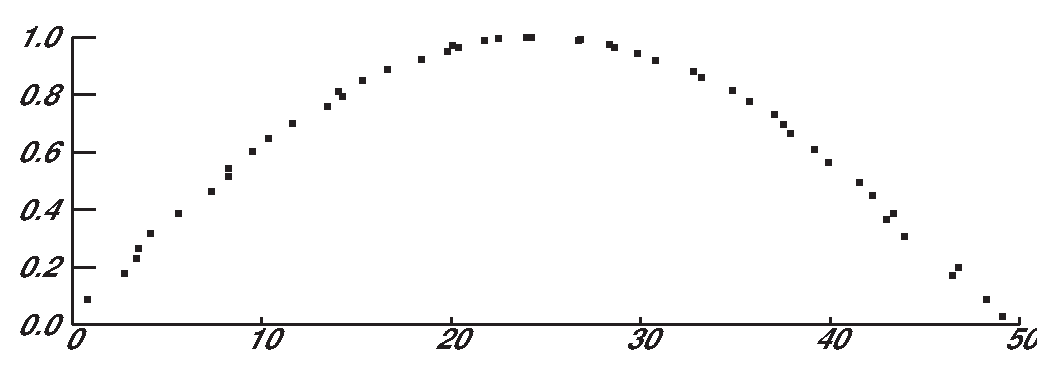
\includegraphics[scale=0.6]{graph_.eps} 
\caption{グラフの例}
\label{figure:graph}
\end{figure*} 

図\ref{figure:graph}は,2段抜きの図の例である.2段抜きの図を挿入するとき
には,\verb|\begin{figure}|の代わりに\verb|\begin{figure*}|とし,
\verb|\end{figure*}|で終わるようにすればよい.同様に\verb|table|について
も\verb|*|をつけることで2段抜きにできる.

ただし2段抜きの図や表は,\LaTeX によって別のページに移動して張り付けられ
てしまうことが多いので注意が必要である.

\subsection{キャプション,図表中のテキスト}
図表のキャプションについては,図の場合は図の下,表の場合は表の上に配置する.

図中の注釈などのテキストはキャプションと同じかやや小さいサイズ,読みやすさの観点ではゴシック系フォントの利用が望ましい.表のテキストもキャプションと同じかやや小さいサイズが望ましい.

\subsection{図作成上の注意点}
原稿を作成する場合,著者は必ず仕上がりを確認し,図が鮮明に,意図した場所に出
力されることを確認する.特に,次の点に留意すること.
\begin{itemize}

 \item 画面キャプチャした画像を使って図を作る際,非可逆圧縮を使わないこ
       と.画面キャプチャした画像をファイルに保存する場合には,保存形式
       として非圧縮形式(BMP等)または可逆圧縮形式(GIF,PNG等) を用いる.

 \item 図に文字を使って注釈を書き込む場合,極力,アウトラインデータの文
       字を用いること.ビットマップデータの文字を用いた場合,文字の輪郭
       がギザギザに見える.
\end{itemize}

\subsection{数式の例}
数式の書き方の詳細はIEEE style manual\cite{IEEE2014}を参照.長すぎる数式は適宜改行し,余白にはみ出さないようにすること.

式(\ref{eqn:sum})は数式の例である.

\begin{equation}
\sum^{N}_{n=1}n = \frac{1}{2}N(N+1)
\label{eqn:sum}
\end{equation}

\subsection{節と項の数について}
1つの章の中に節を作るときは必ず複数個の節を作ること.1個しか節を作る必要がないときはそもそも節に分ける必要がない,ということである.同様に,1節の中に1個しか項がない,という場合も章構成を見直す.

良い例)1章→1.1節,1.2節,2章…

悪い例)1章→1.1節,2章…

\section{著作物の利用について}
論文中に掲載する写真,イラストについて,他者の著作物ではないか,肖像権等に問題はないか,など十分に留意し,必要に応じて適切な手続き,記述の追加を行うこと.


\section{むすび}

このサンプルは次の環境を用いて動作を確認した.
\begin{itemize}
\item UNIX用の p\LaTeXe (p\TeX3.1.2)
\item Windows用の p\LaTeXe (p\TeX3.1.3)
\end{itemize}
本スタイルシートが著者諸氏の論文作成に役立つことを期待する.

\section*{謝辞}
シングルブラインド査読のため,謝辞は入れた状態で投稿する.
謝辞の例:本研究はJSPS科研費 JP12345678の助成を受けたものです.


%%
%%	参考文献
%%
% \begin{thebibliography}{1}

% \bibitem{wiss} WISSホームページ.  http://www.wiss.org/.

% \bibitem{aoki1999} H.~Aoki, B.~Schiele, and A.~Pentland.  Realtime
% Personal Positioning System for Wearable Computers.  In
% \emph{Proceedings of the 3rd IEEE International Symposium on Wearable
% Computers}, pp. 37--43, 1999.

% \bibitem{rekimoto2000} 暦本 純一.  まえがき:WISS2000について.  インタラ
% クティブシステムとソフトウェアVIII, pp. i--ii. 近代科学社, 2000.

% \end{thebibliography}

\section{てすと}

てすとてすとてすとてすとてすとてすとてすとてすとてすとてすと.
てすとてすとてすとてすとてすとてすとてすとてすとてすとてすと.
てすとてすとてすとてすとてすとてすとてすとてすとてすとてすと.
てすとてすとてすとてすとてすとてすとてすとてすとてすとてすと.
てすとてすとてすとてすとてすとてすとてすとてすとてすとてすと.
てすとてすとてすとてすとてすとてすとてすとてすとてすとてすと.
てすとてすとてすとてすとてすとてすとてすとてすとてすとてすと.
てすとてすとてすとてすとてすとてすとてすとてすとてすとてすと.
てすとてすとてすとてすとてすとてすとてすとてすとてすとてすと.
てすとてすとてすとてすとてすとてすとてすとてすとてすとてすと.
てすとてすとてすとてすとてすとてすとてすとてすとてすとてすと.
てすとてすとてすとてすとてすとてすとてすとてすとてすとてすと.
てすとてすとてすとてすとてすとてすとてすとてすとてすとてすと.
てすとてすとてすとてすとてすとてすとてすとてすとてすとてすと.
てすとてすとてすとてすとてすとてすとてすとてすとてすとてすと.
てすとてすとてすとてすとてすとてすとてすとてすとてすとてすと.


文章量が増えると,本文と未来ビジョンが重なるため,重ならないように文章量を調整すること.

\balance %最後の高さを揃えるために必要 (2012/9/27:watanabe, Igarashi)
\bibliographystyle{jwiss}
\bibliography{sample}



%%%%%%%%%%%%%%%%%%%%%%%%%%%%%%%%%%%%%%%%%%%%%%%%%%%%%%%%%%%%%%%%%%%%%
%%%%%%%%%%%%%%%%%%%%%%%%%%%%%%%%%%%%%%%%%%%%%%%%%%%%%%%%%%%%%%%%%%%%%
%% WISS2012では,「未来ビジョン」は以下のように,本文と同様の2段組形式で記載する.
%% 図を用いても良いが,枠のサイズ(縦93mm)を変更してはならない.
%% (WISS2010では,縦118mmでしたのでご注意下さい)

\begin{figure*}[!b]
\setlength{\unitlength}{1mm}\fboxrule=0.5pt

\vspace{-93mm} %% 未来ビジョンの枠が下がってしまうのを防ぐ WIS2012 カメラレディテンプレで追加  (2012/9/27:watanabe, Igarashi)

% 未来ビジョンの枠の描画
\begin{center}
\framebox[0.95\textwidth]{
\begin{minipage}{0mm}\begin{picture}(0,91)(0,0)\end{picture}\end{minipage}
}
\end{center}
\vspace*{-93mm}	% 未来ビジョンの枠の縦幅分だけ戻す

% 未来ビジョンの内容
\newbox\FUTURE
\setbox\FUTURE=\vbox{
\begin{minipage}[b]{0.9\textwidth}
\begin{multicols}{2}	% 二段組にする
\section*{未来ビジョン}
\setlength{\parindent}{10pt}	% 段落先頭の字下げ

% % % % % % % % % % % % % % % % % % % % % % % % % % % % % %
%	   未来ビジョンは,下記に記入して下さい		  %
% % % % % % % % % % % % % % % % % % % % % % % % % % % % % %

\vspace*{-1mm}

% フォントサイズ指定
\normalsize
%\large
%\small\setlength{\baselineskip}{12pt}
%\footnotesize\setlength{\baselineskip}{12pt}

(本行を含む下記の説明を削除してから,記入すること.)

未来ビジョンについては,必須とせず任意とする.論文本体とは別
に,「この研究はどういう未来を切り拓くのか」について,著者の視点からア
ピールしたい点があれば,このような欄を設けて設けて自由に議論してよい.
例えば,「こういう未来社会が到来して欲しいから,我々の研究でこう貢献
していきたい」,「主張が大きすぎて本文中では書きにくかったが,この研究
は,実はこういう気持ちで研究している」,「現在の実装では,小さいトピック
であるかのように誤解を招きやすいが,本当はこういう大きなことを狙って,そ
の第一歩として研究に取り組んでいる」のように,研究の未来,魅力を語る場と
して利用できる.大きさや形状はこのサンプルを目安とするが,この枠内であればある程
度改変してもよいものとする.

てすとてすとてすとてすとてすとてすとてすとてすとてすとてすと.てすとてすとてすとてすとてすとてすとてすとてすとてすとてすと.てすとてすとてすとてすとてすとてすとてすとてすとてすとてすと.てすとてすとてすとてすとてすとてすとてすとてすとてすとてすと.てすとてすとてすとてすとてすとてすとてすとてすとてすとてすと.てすとてすとてすとてすとてすとてすとてすとてすとてすとてすと.てすとてすとてすとてすとてすとてすとてすとてすとてすとてすと.
%% 文章を補う図表を利用してもよい.
\vspace*{5mm}
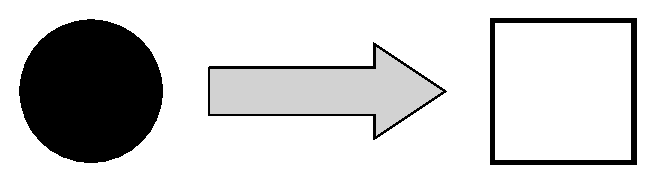
\includegraphics[width=0.95\columnwidth]{vision.eps}
% % % % % % % % % % % % % % % % % % % % % % % % % % % % % %
%	   未来ビジョンは,上記に記入して下さい		  %
% % % % % % % % % % % % % % % % % % % % % % % % % % % % % %

\end{multicols}
\end{minipage}
}

% 未来ビジョンの内容の描画
\newlength{\FUTUREHT}
\setlength{\FUTUREHT}{\the\ht\FUTURE}	% 未来ビジョンの内容の縦幅保存
%\typeout{\the\wd\FUTURE}
%\typeout{\the\ht\FUTURE}
\hspace*{0.045\textwidth}	% 未来ビジョンの内容の横位置調整
\box\FUTURE
%\typeout{\the\FUTUREHT}
\vspace*{-\the\FUTUREHT}	% 未来ビジョンの内容の縦幅分だけ戻す
\vspace*{-10.9mm}		% 微調整

% 未来ビジョンの枠の領域の再確保(これがないと枠が下に沈み込む)
\begin{center}
\fboxrule=0pt
%\fboxrule=2pt	% デバッグ用: コメントアウトをやめて,同じ位置に枠が出るか?
\framebox[0.9\textwidth]{
\begin{minipage}{0mm}\begin{picture}(0,91)(0,0)\end{picture}\end{minipage}
}
\end{center}
\end{figure*}

%%%%%%%%%%%%%%%%%%%%%%%%%%%%%%%%%%%%%%%%%%%%%%%%%%%%%%%%%%%%%%%%%%%%%
%%%%%%%%%%%%%%%%%%%%%%%%%%%%%%%%%%%%%%%%%%%%%%%%%%%%%%%%%%%%%%%%%%%%%
\end{document}
